% Chapter 4

\chapter{Delivering Slide Presentations} % Chapter title
\label{ch:aparecium} % For referencing the chapter elsewhere, use \autoref{ch:name} 

%----------------------------------------------------------------------------------------
\begin{flushright}{\slshape    
Presentation of ideas is conversation \\
carried on at high voltage -- at once \\
dangerous and more powerful.}\\ \medskip
--- \defcitealias{boettinger:1989}{Henry Boettinger}\citetalias{boettinger:1989} \citep{boettinger:1989}
\end{flushright}
%----------------------------------------------------------------------------------------

Presentations are everywhere. We give and sit in on presentations in classrooms, at business meetings, and in conferences. Not surprisingly, presentation technology plays an important role in how we communicate and learn. \\

Electronic slides have become especially popular with standard software PowerPoint and Keynote. While slides allow attractive presentation of visual information, they do not afford some of the basic flexibility that traditional tools such as blackboards provide for pacing, handwriting, content or layout adjustment. \\

In this chapter, we introduce \textbf{Aparecium}, 
%
\marginpar{Aparecium:\\ A charm for revealing invisible ink\cite{rowling1997harry}}
%
a presentation interface that helps presenters deliver flexible and engaging presentations by combining the aesthetics and organization of electronic slides with the spontaneity of inking. In Aparecium, presenters use inking interactions to deliver slide presentations. With inking, presenters can (1) reveal pre-authored content to the audience, (2) make annotations on top of the slide, and (3) adjust the slide layout to create blank space. Pre-authored slides help improve the visual aesthetics and organization of the slides, while inking enables presenters to have flexibility and fine-grained control over the content and pace of the presentation.\\

In a user study comparing Aparecium with baseline presentation tools, we found that our interface generally improves presentation quality without increasing the burden on the presenter at authoring or presentation time. Especially for text-centered or process-driven content, both audiences and presenters preferred presentations delivered using Aparecium.

\section{Introduction}

Presentations are an important component of both classroom and online instruction. 
They allow presenters to communicate concepts by combining visual content with spoken explanations.
As a result, tools for authoring and delivering presentations have a significant influence on how people teach and learn.
Today, the two dominant types of presentation technology are slides and blackboards.\\

Slides allow presenters to refine the appearance and organization of material in advance. As such, they are most convenient for information-rich content like images or detailed diagrams and charts. 
However, pre-authored slides restrict how content can be revealed during the presentation. Rather than displaying all of the slide content at once, which can make it difficult for the audience to know where to focus, presenters often set up animation effects to reveal visual elements incrementally. Since the sequence and granularity of these animations are determined ahead of time, it is difficult to add new content or change the order of reveals during the presentation, for instance, in response to the audience.
%
Animations also display information quickly and hasten the pace of the presentation. Indeed, slide lectures tend to show more information in a shorter period of time than blackboard lectures \cite{lanir2008observing}, potentially making it more difficult for the audience to follow.\\

As an alternative, some presenters prefer to write on physical blackboards or ink on virtual displays in real-time. This presentation style is direct and intuitive, and in contrast to pre-authored slides gives presenters full control over how content is displayed.
%
On the other hand, writing and talking at the same time is cognitively demanding. As a result, bad handwriting and poor layouts (e.g., running out of room while writing) are common in blackboard-style presentations. It is also difficult to incorporate complex visuals since they must be created from scratch during the presentation. This often results in long pauses or rambling, repetitive explanations as presenters focus on drawing or writing.\\

Some presenters blend the two modes of presentation, for example, by projecting slides onto a board and inking on top of them. Recently, PowerPoint and Keynote, also allow presenters to ink over electronic slides in presentation mode. However, in these approaches, the ink and underlying slides are treated as completely separate layers of content that retain their individual drawbacks. 
%
The slide content remains fixed and inflexible while real-time inking still requires the user to draw carefully albeit with the help of the slide content as a reference.\\

To address these limitations, we propose Aparecium, a presentation interface that combines the advantages of slides and inking.
%
In Aparecium, presenters use pre-authored slides to prepare the presentation content. However, instead of specifying animations beforehand, presenters use inking interactions to flexibly display the content on demand. By inking, presenters can control the pace at which pre-authored material is revealed, as if writing in real-time. At the same time, they do not have to worry about writing neatly or carefully arranging all the visual elements on the screen. Our system also allows improvised annotations and enables presenters to create blank space inside the slide to insert new content during the presentation. Aparecium supports all of these functions as modeless interactions.\\

We evaluate our interface from the perspective of presenters and the audience and compare Aparecium against two baselines, representing conventional slide and inking tools. Presenters found Aparecium easy to use for preparing and delivering presentations. They were also generally pleased with the quality of the presentation produced using our interface. 
%
Overall preferences between presentation interfaces depended on the type of content.
%
Both presenters and audience members clearly preferred Aparecium for text-heavy, process-driven material (e.g., explaining algorithms or mathematical derivations), and rated our system as comparable to the baseline slide interface for presenting complex, multi-part diagrams. \\

To summarize, this chapter presents the following contributions:

\begin{itemize}
  \item The design and architecture of a new presentation interface, Aparecium, that combines inking with pre-authored slides.
\item A set of modeless inking interactions that analyze the underlying slide content to help presenters reveal, annotate, and create extra space during a presentation.
  \item An evaluation from the perspective of presenters and the audience that compares Aparecium against two baseline interfaces.
%  \item Based on formative interviews and observations from our user study, we discuss design directions for future presentation interfaces. 
\end{itemize}


%----------------------------------------------------------------------------------------

\section{Previous Work}

\subsection{Presentation Software.} The vast majority of presentations today are created with WYSIWYG slide authoring software like PowerPoint \cite{powerpoint2017}, Keynote \cite{keynote2017} and Google Slides \cite{googleslides2017}. 
%
While these tools provide a broad range of content creation features, including the ability to add animation effects to slide elements, 
they offer limited flexibility or control at presentation time. 
%
Presenters can only advance linearly through the predefined sequence of animations and slide transitions.

\subsection{Nonlinear Presentations.} 
To address this shortcoming, research investigated how to support nonlinear paths though a presentation. Moscovich et al \cite{moscovich2004customizable} organize slides into nested directed graphs and allow presenters to choose between multiple paths on the fly. Similarly, Drucker et al. \cite{drucker2006comparing} suggest a method to compare and manage multiple slide presentation paths. Fly \cite{lichtschlag2009fly} and CounterPoint \cite{good2002zoomable} allow spatial navigation by embedding slides on an infinite canvas and employing zooming user interfaces (ZUIs). Prezi \cite{prezi2017} is a commercial, online platform for authoring zoomable presentations. Whereas these work focuses on navigating between slides or the presentation as a whole, the interactions presented in this chapter provide flexibility and control within each slide.

\subsection{Controlling Presentations.} 
Other work explores alternative techniques to control slide presentations. Palette \cite{nelson1999palette} uses physical cards to provide random access to slides, Baudel and Beaudouin-Lafon \cite{baudel1993charade} propose hand gestures, and Cheng and Pulo \cite{cheng2003direct} use an infrared laser pointer to control presentations. Cao et al. \cite{cao2005evaluation} perform a systematic user study comparing different interaction techniques, including hand gestures, laser pointer and standard mouse/keyboard input. We suggests inking interactions as the main mode to present slides.

\subsection{Inking on Digital Documents.} 
Many systems \cite{yoon2014richreview, marshall1999collaborating, hardock1993marking} support digital inking to make annotations on top of documents. Perhaps most similar in spirit to Aparecium are systems that integrate digital ink with electronic slides. Anderson et al.~\cite{anderson2007classroom} propose Classroom Presenter, a distributed presentation system that allows instructors and students to share digital ink on top of electronic slides. Recently, PowerPoint and Keynote added support for presenters to ink in presentation mode as well. SMART is another commercial system that supports inking and projected material using an interactive whiteboard \cite{smarttech2017}. While all of these systems combine slides with inking, the underlying slide content remains inherently separate from the ink on top. In contrast, in our system, presenters use ink to reveal underlying slide elements in a flexible, fine-grained way at presentation time.

\subsection{Beautifying Ink.} To further assist freeform digital inking, researchers have experimented with different methods to beautify the user's ink strokes. Beautification is applied to meet the requirements of specific scenarios, such as geometric diagrams \cite{igarashi1998pegasus, hse2005recognition, fivser2015shipshape}, hand-drawn pictures~\cite{xie2014portraitsketch, limpaecher2013}, handwriting \cite{zitnick2013handwriting} or mathematical diagrams~\cite{laviola2007mathpad}. Aparecium does not modify the user's ink stroke per se, but it achieves a similar effect by making the ink stroke disappear gradually and revealing the underlying pre-authored slide content instead.

%----------------------------------------------------------------------------------------

\section{Design Principles}
\subsection{Current Practices and Needs}
To learn about current practice and unsupported needs in presentation technology, we conducted in-depth interviews with 5 university lecturers, 8 graduate student TAs, 5 undergraduate students, and 5 online lecturers, each from multiple institutions and with varied experiences in giving and listening to presentations. The interviews were semi-structured and covered 1) the methods of presentations they used, 2) in what settings they prefer slides versus inking, 3) challenges of currently available technologies and what they would like to see in future presentation systems. We also consulted existing literature comparing different types of presentation software. From this analysis, we summarize the key findings that informed the design of our system.

\subsubsection{Flexibility in presentations is preferred for interactive or informal settings.} For settings such as research conferences or business meetings with tight time constraints and little room for audience interaction, people prefer to give highly scripted presentations with electronic slides. However, for settings such as lectures, tutoring sessions, or brainstorming meetings, presenters like to have some flexibility and often use inking as part of their presentations. Common strategies include using a blackboard or projecting slides/transparencies onto a board and inking on top of them. Several lecturers purposefully leave blank spaces on their slides to fill in by inking during the lecture. 

\subsubsection{Presenters want flexibility over prepared contents rather than complete improvisation.} 
Even for informal settings, presenters have the bulk of the content planned and prepared beforehand, in the form of lecture notes, worksheets or slides. Thus, the type of flexibility that presenters want is the ability to make small-scale adjustments on-the-fly, such as omitting part of the content, adding minor changes such as a line of text or annotations, or changing the order of the contents. Inking is often used to this effect. 

\subsubsection{Pacing is important and context dependent.} 
The choice of tool also affects the pace of the presentation. Electronic slides are useful for displaying information quickly, which may explain why presenters prefer them for time-constrained settings. Inking takes time, but it allows presenters to have fine-grained control over the pace of the presentation. Depending on the subject matter, the pace of real time writing also makes it easier to follow for the audience. For example, when describing sequential processes like solving a math problem or explaining a complex diagram, both presenters and viewers find it more effective to write them out step-by-step in real-time. Slide animations can simulate this effect, but setting up fine-grained animations is tedious. As a result, animated presentations typically include a very coarse set of discrete steps. 

\subsubsection{Visual aesthetics matter but are difficult to achieve with inking.} 
Both as a presenter and as an audience, people frequently mentioned better visual aesthetics as an advantage of slides over inking. Presenters are often not satisfied with or even embarrassed by their own handwriting. They pointed out that it is even more difficult to write while talking at the same time. Even small operations, such as changing the pen color, seem burdensome during the lecture, as noted by Anderson\cite{anderson2004study}. 
From a viewing perspective, people like the legibility and organization that pre-authored slides provide. As \cite{frey2002learners} also mention, sometimes audiences even felt that lecturers are better organized when they present using electronic slides. 

\subsection{Design Goals}
The above findings highlight the complementary attributes of electronic slides and inking. While slides are typically more organized and aesthetically pleasing, inking offers greater flexibility and fine-grained control at presentation time.
%
Our aim is to develop a presentation interface that combines the advantages of both existing technologies without increasing the burden on the presenter at authoring and presentation time.
%
More specifically, our system should achieve the following design goals. The first two goals are concerned with improving the presentation quality, while the last goal involves reducing the presenters' effort. 

\subsubsection{Maximize organization and aesthetics through pre-authored contents.} 
In order to improve presentation quality, we want to take full advantage of contents that presenters prepare beforehand. Pre-authored contents can help achieve visual aesthetics. It also \emph{forces} the presenter to organize the presentation ahead of time. 
 
\subsubsection{Maximize flexibility and fine-grained control during presentation delivery.} Presenters should have fine control over what visual content to present, and also when, how much, and how fast to present them. Moreover, these decisions need not be made ahead of time; instead, presenters should be able to implement and adjust them while delivering, according to the content and audience. 

\subsubsection{Minimize presenter effort during delivery as well as during preparation.} 
We want to give presenters more control, but without increasing their burden. Interactions during delivery should be as simple and natural as possible. Similarly, preparation itself should not take more effort than, for example, authoring regular slides. Moreover, presenters should be allowed to focus more on preparing the content itself rather than, for instance, spending time to setup animations effects for delivery. 


%----------------------------------------------------------------------------------------

\section{The Aparecium Interface}

Based on these design goals, we developed Aparecium, a presentation system that combines electronic slides with inking interactions. With Aparecium, presenters pre-author slides to organize and refine the visual aesthetics of their material. Unlike traditional electronic slides, presenters do not specify beforehand when, how, or in which order the visual elements in the slide will appear via scripted animation effects. Instead, they simply specify which elements will be displayed to the audience immediately (background) versus which elements will be hidden and then revealed in real time (foreground).\\ 

The key innovation of Aparecium is in how presenters deliver the pre-authored content.  The main mode of interaction at presentation time is inking, but instead of just adding strokes to the slide, inking supports three functions depending on the context: (1) If the presenter inks over hidden elements, it reveals the pre-authored element to the audience. (2) If the presenter inks over empty space or over revealed elements, ink strokes are added on top of the slide. (3) Finally, if the presenter holds down the pen after drawing a stroke, the user can adjust the slide layout to create blank space.\\ 

Inking allows presenters to have flexibility and fine-grained control over when, how much, and how fast to reveal elements on the slide.
%
At the same time, the ability to reveal pre-authored content allows presenters to not worry about writing or drawing neatly.
%
Presenters can also add extra writing or annotations on top of pre-authored elements, and create blank space if necessary. 
%
All of these interactions are implemented as modeless pen interactions.\\

Here we elaborate on slide authoring and inking in our system.
%\begin{figure*}
%  \centering
%  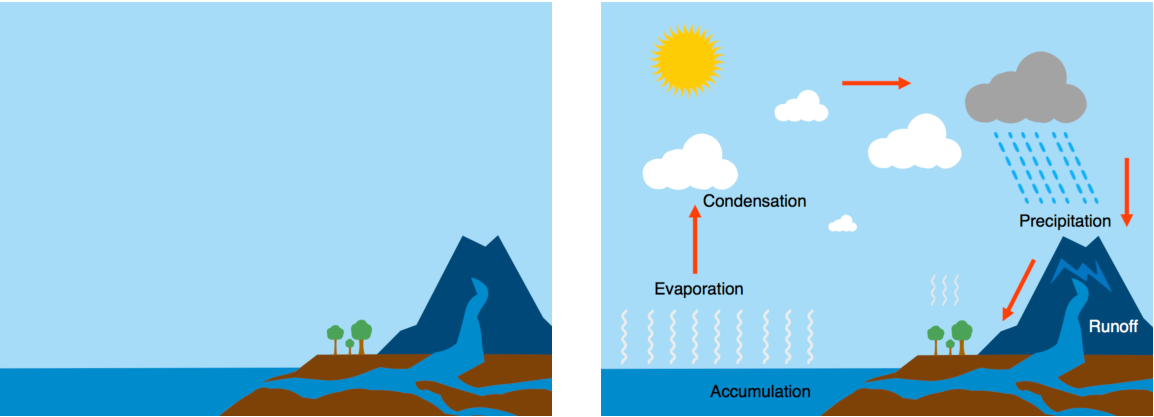
\includegraphics[width=2.0\columnwidth]{figures/watercycle}
%  \caption{}~\label{fig:watercycle}
%\end{figure*}
\subsection{Slide authoring}
Slides in Aparecium can be authored using any existing slide presentation software (e.g., PowerPoint, Keynote, GoogleSlides). They can include typed text or images, as well as, hand drawn ink strokes. Instead of specifying animation effects on these slide elements, presenters separate them into two layers for each slide. The background layer is always visible and it is what the audience sees initially. The foreground layer is initially only visible on the presenter view, but presenters can reveal parts of it to the audience during delivery. Presenters also have the option of preparing a third layer, the notes layer, which is only visible on the presenter view and acts as transparent speaker notes placed on top of the slides. Layers in Aparecium are represented as bitmap images. (Figure~\ref{fig:slidelayers})

\begin{figure*}[h!]
    \centering
    \begin{subfigure}[t]{0.31\textwidth}
        \centering
        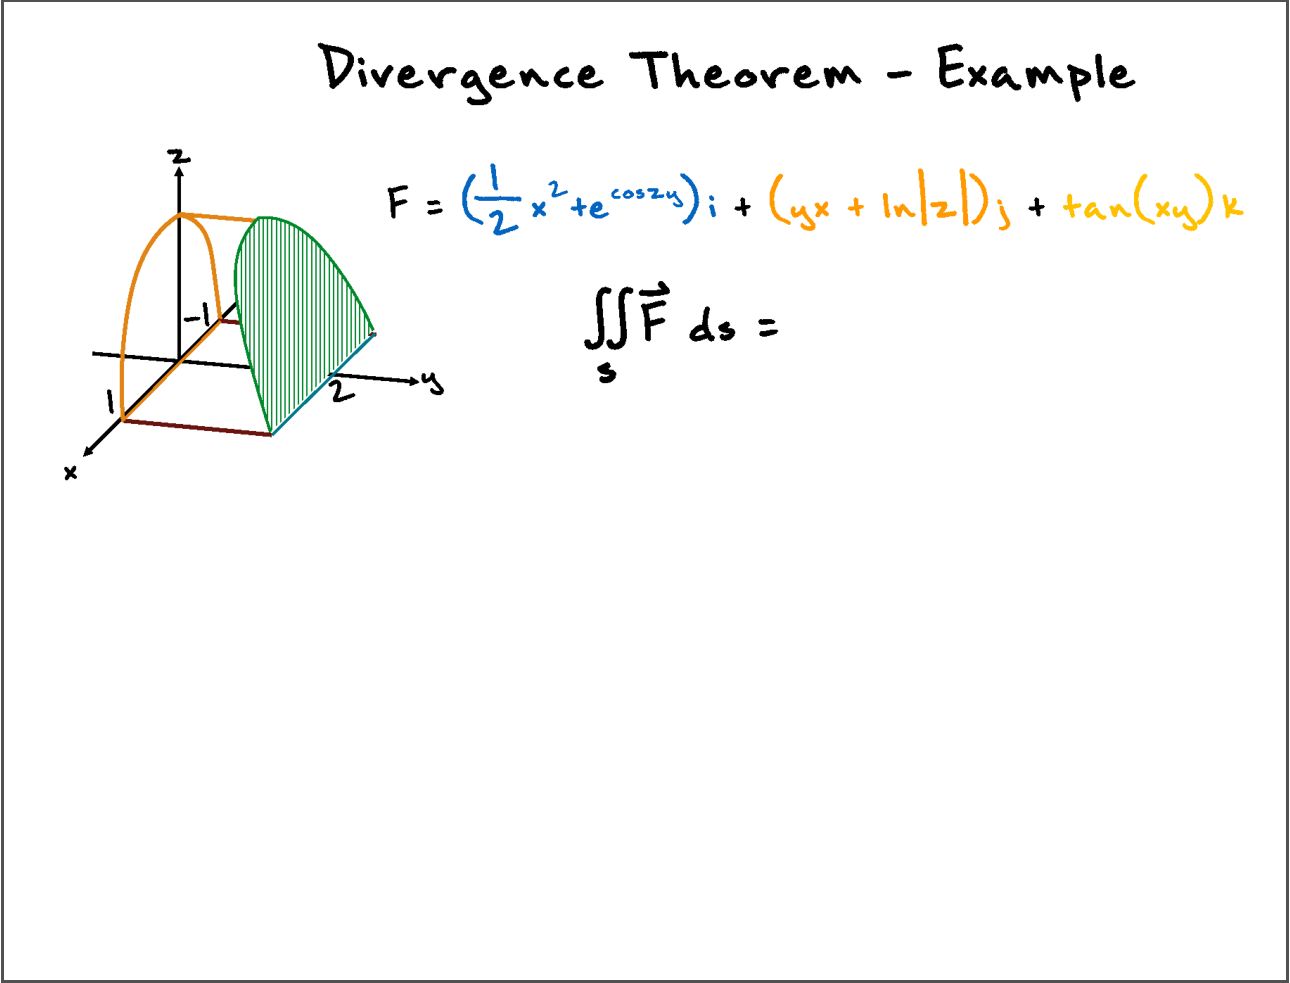
\includegraphics[width=1\columnwidth]{figures/videoslide1}
\captionsetup{font=footnotesize}
        \caption{Background (Audience View)}
    \end{subfigure}%
    ~ 
    \begin{subfigure}[t]{0.31\textwidth}
        \centering
        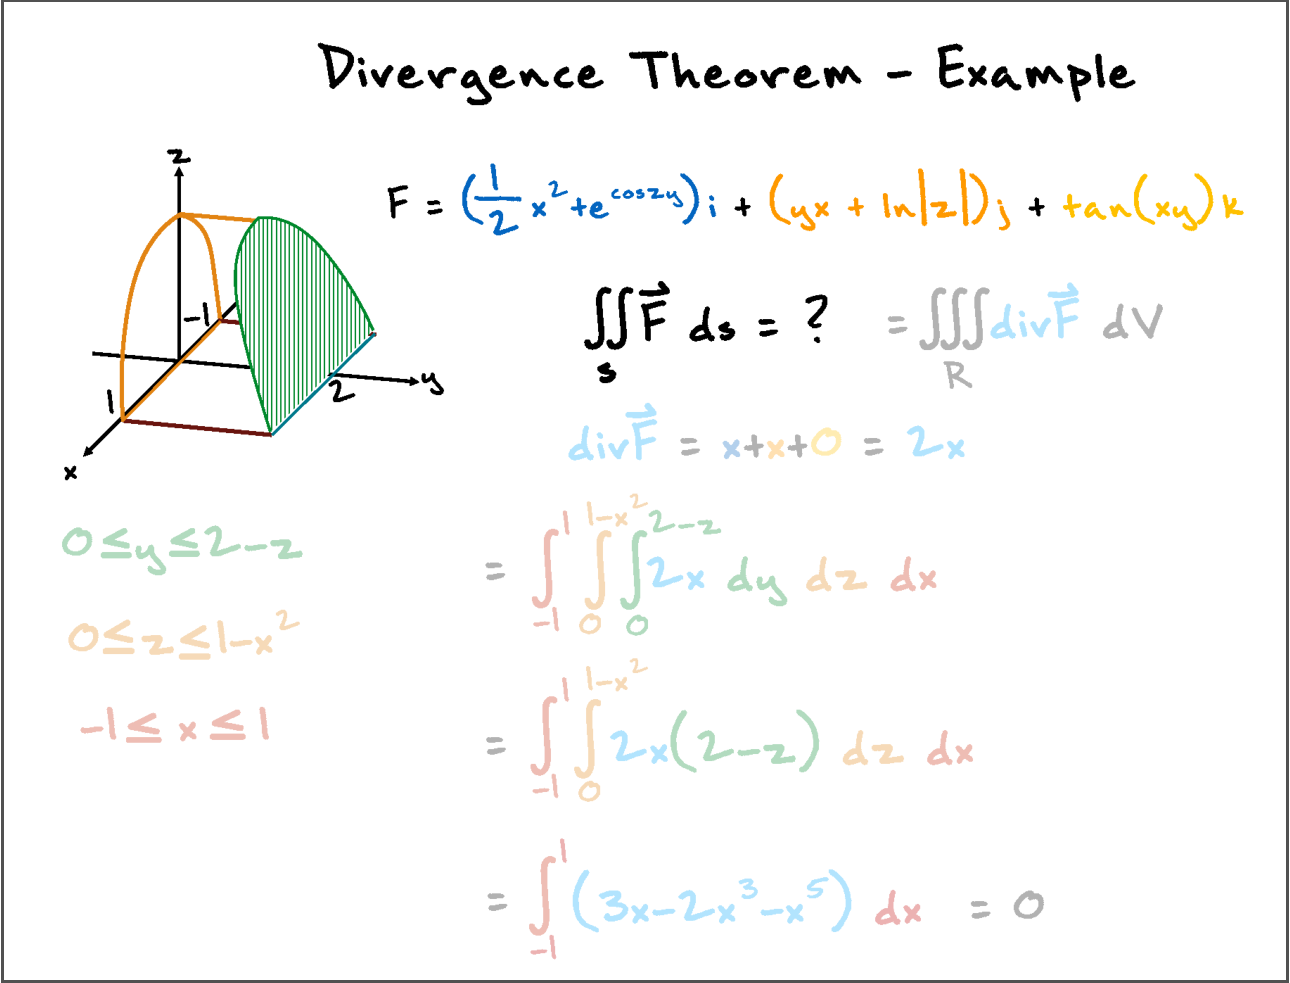
\includegraphics[width=1\columnwidth]{figures/videoslide2}
        \captionsetup{font=footnotesize}
        \caption{Background + Foreground\\ (Presenter View)}
    \end{subfigure}
    ~
        \begin{subfigure}[t]{0.31\textwidth}
        \centering
        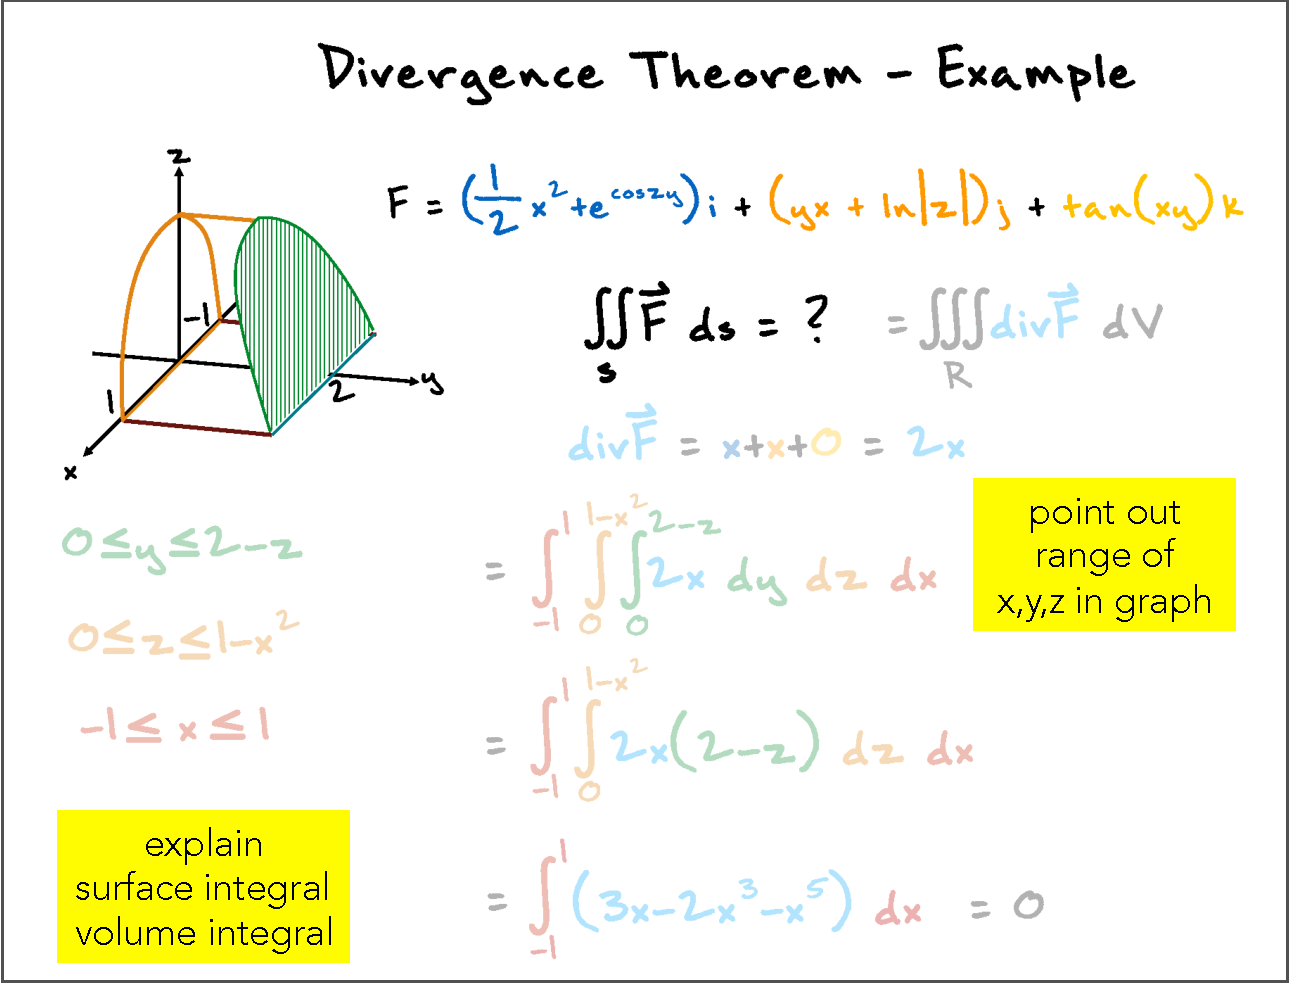
\includegraphics[width=1\columnwidth]{figures/videoslide3}
        \captionsetup{font=footnotesize}
        \caption{Background + Foreground + Notes}
    \end{subfigure}
    \caption{Slide Layers in Aparecium. Slides are separated into foreground and background layers. \textbf{(a)} The background layer is always visible and it is what the audience sees initially. \textbf{(b)} The foreground layer is initially only visible on the presenter view, and is faded to distinguish it from the background. Presenters can reveal parts of it to the audience during delivery. The revealed parts appear on the audience view and becomes unfaded on the presenter view. \textbf{(c)} Optionally, presenters can also have the notes layer, which is only visible on the presenter view and acts as transparent speaker notes placed on top of the slides. }
    \label{fig:slidelayers}
\end{figure*}

\subsection{Inking during delivery}
%
Aparecium enables robust, modeless inking operations at presentation time by leveraging the structure of the pre-authored slide content. Each of the three inking functions uses this structure in different ways. 
\subsubsection{Reveal}
To reveal hidden foreground content to the audience, the presenter inks over the relevant portion of the foreground layer.
%
At the end of each stroke, the system computes a subset of the surrounding foreground pixels to display. 
%
For each point, $s_i$ on the stroke, the closest foreground pixel, $p_i$ is computed. If the distance between $p_i$ and $s_i$ is within a threshold $\alpha$, a flood-fill is performed starting from $p_i$ to neighboring foreground pixels. The value of $\alpha$ determines how precisely the user has to ink in order to reveal the underlying content. Since presenters can be more precise when they are inking slowly versus when they are inking quickly, $\alpha$ is set to vary proportionally to inking velocity, $v$:
%
\begin{equation}
\alpha = 0.02v+10
\end{equation}
where both $\alpha$ and $v$ are measured pixel space.\\
 
The extent of the flood-fill is limited by two additional thresholds $\beta$ and $\gamma$ on (1) the distance from $p_i$, and (2) the color difference from $p_i$ in Lab space. 
%
To give presenters finer-grained control over the extent of the reveal, $\beta$ and $\gamma$ also vary according to the velocity of the presenter's ink stroke:\\ 
\begin{equation}
    \beta = min(0.01v+5,\;40)
\end{equation}
%
\begin{equation}
\gamma = 0.05v+10
\end{equation}

Our algorithm has several important properties. Bounding the flood-fill with $\beta$ and $\gamma$ ensures that the revealed content is localized around the user stroke and prevents ``bleeding'' across regions with very different colors.
%
In addition, modulating $\beta$ and $\gamma$ based on the stroke velocity allows presenters to reveal with different levels of precision. 
%
To show a small piece of content, the presenter can ink slowly over the relevant foreground region. This interaction is useful when the presenter wants to simulate writing in real-time, or needs to reveal a specific element in a dense slide. For example, in Figure~\ref{fig:inkreveal}(a), the presenter slowly writes out a part of the integral $\int_{-1}^{1}\int_{0}^{1-x^2}\int_{0}^{2-z}2x$, while explaining each of the domains.
%
In other situations, users may want to reveal larger pieces of content more efficiently. For example, in Figure~\ref{fig:inkreveal}(c), the presenter reveals all of $dxdydz$ at once to complete the equation. In this case, users can ink quickly and roughly (e.g., by scribbling) over a foreground region.

\begin{figure}[h!]
    \centering
    \begin{subfigure}[t]{0.4\columnwidth}
        \centering
        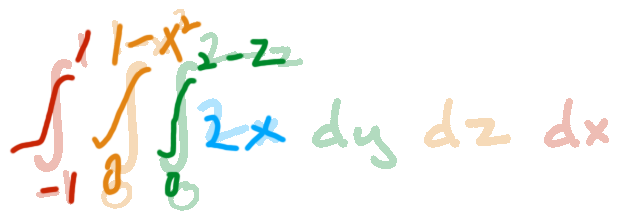
\includegraphics[width=1\columnwidth]{figures/slowink_presenter}
                \captionsetup{font=footnotesize}
\caption{Slowly writing over a portion of the equation (Presenter View)}
    \end{subfigure}%
    ~ ~
    \begin{subfigure}[t]{0.4\columnwidth}
        \centering
        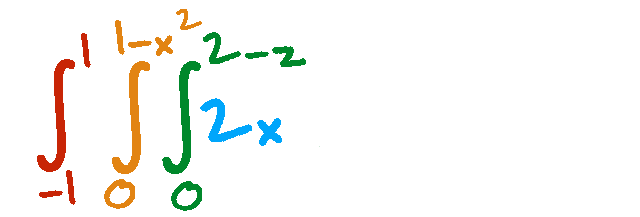
\includegraphics[width=1\columnwidth]{figures/slowink_audience}
                \captionsetup{font=footnotesize}
\caption{After reveal \\ (Audience View)}
    \end{subfigure}
         ~   ~
      \begin{subfigure}[t]{0.4\columnwidth}
        \centering
        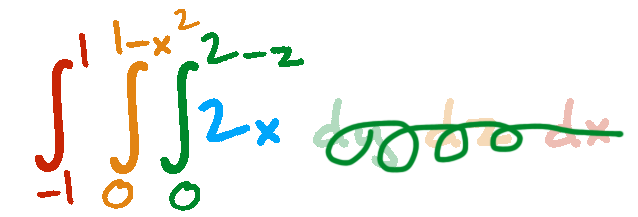
\includegraphics[width=1\columnwidth]{figures/fastink_presenter}
                \captionsetup{font=footnotesize}
\caption{Quickly scribbling over rest of the content (Presenter View)}
    \end{subfigure}%
    ~ ~
    \begin{subfigure}[t]{0.4\columnwidth}
        \centering
        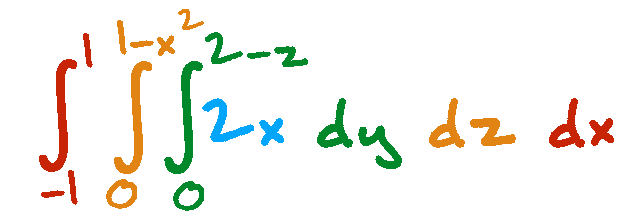
\includegraphics[width=1\columnwidth]{figures/fastink_audience}
                \captionsetup{font=footnotesize}
\caption{After reveal (Audience View)}
    \end{subfigure}
    \caption{Inking to reveal. Presenter inks over foreground content to reveal it to the audience. Presenter can either \textbf{(a)} ink over slowly to simulate writing in real-time, or \textbf{(b)} scribble over quickly to reveal larger portions efficiently. \textbf{(c), (d)} In both cases, the relevant portion of the foreground layer is revealed to the audience and replaces the presenter's original ink strokes.}
    \label{fig:inkreveal}
\end{figure}

\subsubsection{Annotate}
Presenters sometimes add new (i.e., unauthored) information to a slide on-the-fly during a presentation.
%
For example, a lecturer may circle an important concept for emphasis, explicitly label part of a diagram, or even add a whole new line of equation. 
%
To make such annotations in Aparecium, the presenter simply inks over empty (or already revealed) pixels on the foreground layer. If less than 10\% of the $p_i$s are within the $\alpha$ threshold of an unrevealed foreground pixel, the system treats the stroke as an annotation. To ensure that the annotation stands out from the surrounding slide content, Aparecium computes the average color of the slide around the stroke and sets the ink to a complementary color. (Figures~\ref{fig:annotate} and \ref{fig:space}c). 

\begin{figure}[h!]
    \centering
    \begin{subfigure}[t]{0.5\columnwidth}
        \centering
        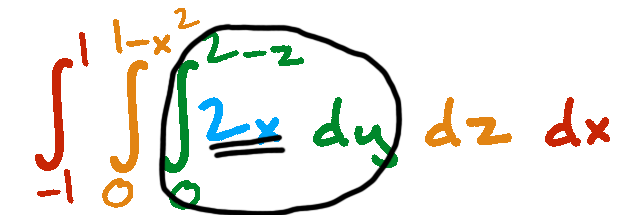
\includegraphics[width=1\columnwidth]{figures/annotate_presenter}
                        \captionsetup{font=footnotesize}
        \caption{Before auto-coloring}
    \end{subfigure}%
    ~ 
    \begin{subfigure}[t]{0.5\columnwidth}
        \centering
        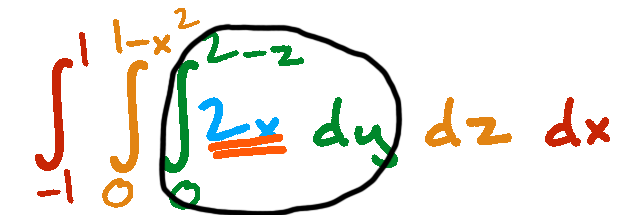
\includegraphics[width=1\columnwidth]{figures/annotate_audience}
                        \captionsetup{font=footnotesize}
\caption{After auto-coloring}
    \end{subfigure}
    \caption{Inking to annotate. \textbf{(a)} Presenter inks over already revealed content to make annotations. \textbf{(b)} To ensure that the annotation stands out from the surrounding slide content, Aparecium computes the average color of the slide around the stroke and sets the ink to a complementary color. In this case, the underlines below the cyan $2x$ is set to orange.}
    \label{fig:annotate}
\end{figure}

\subsubsection{Create Space}
In some cases, presenters may want extra space to insert new content in a slide, for example, to add an item to an existing list, a word in a sentence, or an extra line of explanation. These situations can arise as a result of a mistake in the preparation phase (e.g., the presenter forgets to list an item), as well as from presenter-audience interaction (e.g., the audience requests extra explanation). Aparecium allows presenters to create empty space from ink strokes. First, the presenter draws a curve where the empty space should be created. At the end of the curve, if the presenter holds down the pen for more than 0.5 seconds, the curve turns into a red dashed stroke, indicating that the presenter can start expanding the space around the curve. As the presenter moves the pen along one of the axis-aligned directions, empty space is created and expanded from the curve in that direction.  As the space grows, the foreground content shifts accordingly. (Figure~\ref{fig:space}).

%
\begin{figure}[h!]
    \centering
    \begin{subfigure}[t]{0.48\columnwidth}
        \centering
        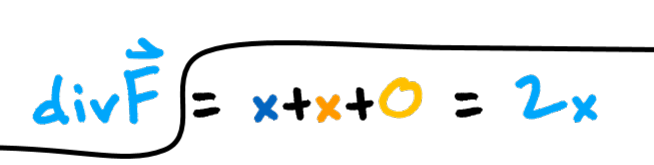
\includegraphics[width=1\columnwidth]{figures/create_space1}
                       \captionsetup{font=footnotesize}
 \caption{Presenter draws a stroke where empty space should be created and holds the pen down (0.5sec)}
    \end{subfigure}%
    ~ 
    \begin{subfigure}[t]{0.48\columnwidth}
        \centering
        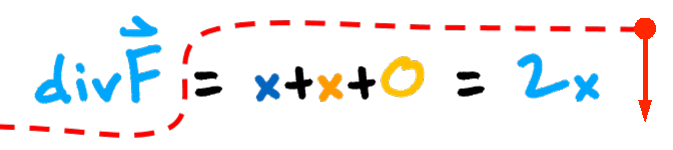
\includegraphics[width=1\columnwidth]{figures/create_space2}
                       \captionsetup{font=footnotesize}
 \caption{The stroke turns into a space-expansion curve. Empty space is created by expanding the curve along the direction of the pen movement and shifting the foreground content accordingly.}
    \end{subfigure}
    ~
        \begin{subfigure}[t]{1\columnwidth}
        \centering
        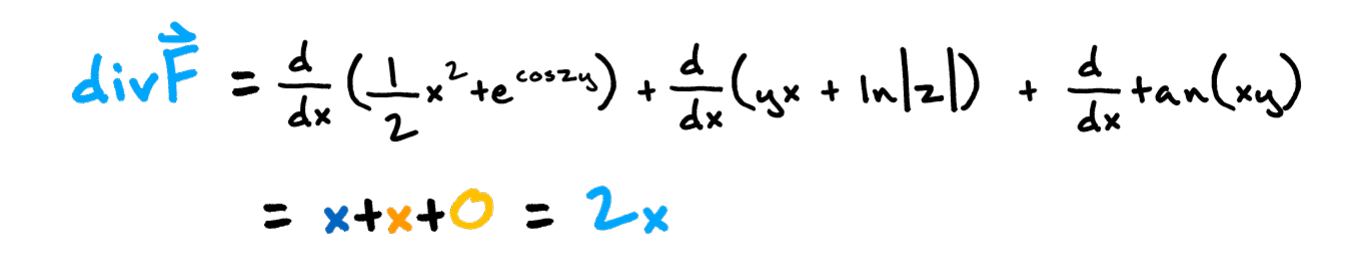
\includegraphics[width=1\columnwidth]{figures/create_space3}
                        \captionsetup{font=footnotesize}
\caption{Presenter inserts annotations in the newly created space }
    \end{subfigure}  
    \caption{Creating space and annotating.}
    \label{fig:space}
\end{figure}
%
As space is created, the slide area grows and scrolling is automatically enabled. Users can also zoom out to fit the slide in a single view.
%----------------------------------------------------------------------------------------

\section{User Evaluation}

We evaluate Aparecium from the perspective of presenters and the audience. We assess the ease of use of the interface from the presenters' point of view, and rate the presentation quality from both the presenters' and the audiences' perspective.\\

To better understand the benefits of our interface, we compared Aparecium against two baselines. The first baseline (\textbf{BaselinePPT}) represents conventional electronic slide tools.
%
We use Microsoft PowerPoint and allow presenters to apply animation effects (but no inking) during the presentation.
%
The second baseline (\textbf{BaselineInk}) represents standard ``blackboard-style'' presentation tools that allows users to ink in real-time during the presentation.
%
For this condition, we also use Microsoft PowerPoint but only allow users to pre-author and deliver content via inking.\\

We hypothesized that different types of content would lend themselves to different presentation styles. We compare three different types of content: (1) a text-centered slide, explaining the derivation of the quadratic formula \textit{(Derivation)}, (2) a diagram-centered slide, describing the hydrologic cycle  \textit{(WaterDiagram)}, and (3) a typical PPT style slide with bullet points and images listing different carpentry tools \textit{(BulletPoints)}. Using PowerPoint, we pre-authored a single page slide for each of these content types (Figure~\ref{fig:studyslides}).\\
%
\begin{figure}[h!]
    \centering
    \begin{subfigure}[t]{1\columnwidth}
        \centering
        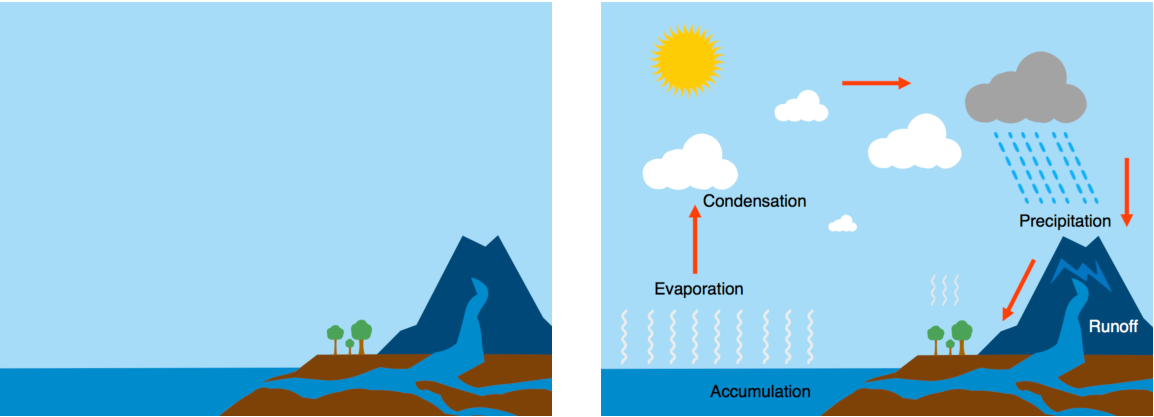
\includegraphics[width=1\columnwidth]{figures/watercycle}
        \captionsetup{font=footnotesize}\caption{\textit{WaterCycle} slide background (left) and foreground (right)}
    \end{subfigure}
    ~ 
    \begin{subfigure}[t]{0.48\columnwidth}
        \centering
        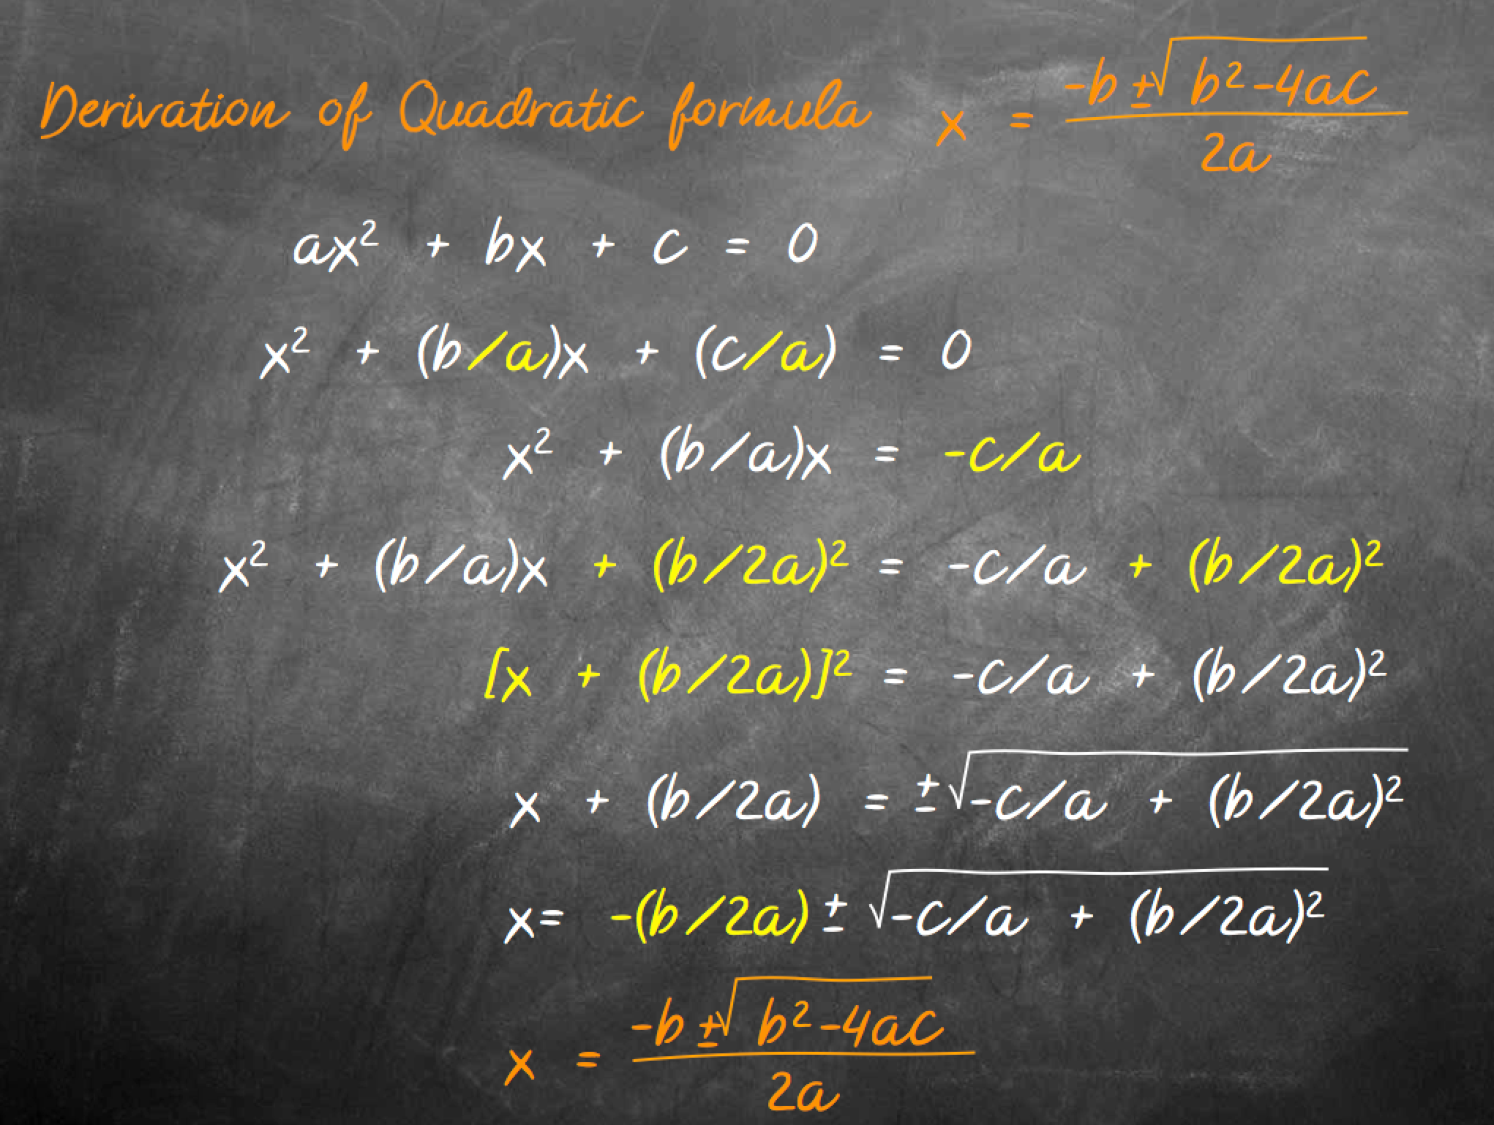
\includegraphics[width=1\columnwidth]{figures/quadformula}
        \captionsetup{font=footnotesize}\caption{\textit{Derivation} slide}
    \end{subfigure}  
    ~
    \begin{subfigure}[t]{0.48\columnwidth}
        \centering
        
\includegraphics[width=1\columnwidth]{figures/tools}
        \captionsetup{font=footnotesize}\caption{\textit{BulletPoints} slide}
    \end{subfigure}  
    \caption{Evaluation slides}
    \label{fig:studyslides}
\end{figure}

To reduce the preparation effort for all three presentation tool conditions, we separated each slide into foreground and background elements, which are shown in our supplemental materials. For the BaselinePPT condition, we leave the individual PowerPoint elements (e.g., arrows, text boxes containing individual lines of equations, images) ungrouped to make it easier for users to author fine-grained animations. 

\subsection{Study 1: Presenter Perspective}
In our first study, we asked participants to present each of the three content types using the three different presentation tool conditions. 
%
For each content type, participants were given the pre-authored, pre-segmented slide. 
They received verbal and written explanations of the material, and a printout of the complete slide contents (both foreground and background layers). They were given time to familiarize themselves with this material and to set up the slide before the presentation.\\

In the BaselinePPT condition, participants could add animation effects to reveal or emphasize the foreground elements. For the BaselineInk condition, the slide only contained background elements. Participants were free to write additional content into the slide as part of their set up, which is analogous to blackboard lecturers writing on the board before class. For Aparecium, participants could also write additional content on top of the background, or they could choose to make some of the foreground elements visible (effectively moving those elements into the background layer). For simplicity, we omitted the space creating functionality in the evaluation. \\

After the setup phase, participants used one of the three tool conditions to deliver the presentation. 
%
To simulate a real presentation, participants were asked to pretend that their presentation was being broadcast live as a webcast. At the end of each trial, we showed the user a screen recording of their presentation and asked them to self-rate their own presentation, this time pretending that they were students trying to learn the subject. Presenters also completed a questionnaire where they rated how easy it was to prepare and deliver presentations using each of the tools. All ratings were done on a 5-point Likert scale.\\

We recruited 12 graduate students from 8 different universities (ages 21 to 31). All of the partcipants were familiar with the PowerPoint interface. We used a within-subject design, where each participant delivered presentations on each interface. We kept the task order fixed and counter-balanced the order of the presentation tools to obtain an equal distribution of task-tool pairs.
%

\subsection{Study 2: Audience Perspective}
In our second study, we recruited a separate set of participants to vote on presentations delivered using each interface.
%
While we considered comparing the output presentations from the first study, we found that there was too much variation in quality between the results. Since presenters were not forced to follow fixed scripts, there were significant differences in length and detail. In addition, the presenters spoke with varying levels of enunciation and enthusiasm (not to mention different accents).
%
Thus, we ourselves produced a new set of more comparable presentations
using the slides from the first study.
%
To make the comparison as fair as possible, we used a fixed script for each content type.
We also analyzed the output presentations from the first study, and used them as a reference when creating our own versions. 
%
For example, for the BaselinePPT condition, we reproduced the granularity and order of animations that we observed in the user-created presentations.
%a
In the BaselineInk condition, we followed the typical ordering of the inked contents and chose similar ink colors. We also recorded the presentations so that the silent pauses in between inking periods were similar (or shorter) than those produced in the first study. 
%
Finally, for Aparecium, we used a similar reveal order, combination of slow tracing versus fast scribbling, and on-the-fly ink annotations as most participants. 
%
In general, presenters from the first study employed similar approaches to inking or animation so it was straightforward to extract common qualities. For the few cases, where participants varied in their approach, we selected an approach that we deemed to produce better quality (e.g., finer-grained animations, use of different ink colors).\\
 
We recruited 36 undergraduate and graduate students from multiple universities to rate the presentations. For each content type, participants watched recordings of three presentations delivered using each interface, and voted for the most engaging presentation. 

\subsection{Findings and Discussion}
Overall, presenters found Aparecium easy to use for setting up and delivering presentations. They were satisfied with the quality of the presentations recorded using our interface, and emphasized that the appearance of real time inking had an engaging effect. 
Preferences between the presentation tools depended on the content type. Participants in both studies (i.e., presenters and viewers) preferred Aparecium for text-centered or process-driven content. \\

Given the size and exploratory nature of our study, we use descriptive statistics to summarize the Likert responses from Study 1. Below we discuss each of our findings in more detail.\\

\subsubsection{Aparecium makes it easier to prepare slides.}
Presenters found it easiest to set up the slides using our interface, followed by BaselineInk and then BaselinePPT (Figure~\ref{fig:likert}). 
%
\begin{figure}[h!]
    \centering
        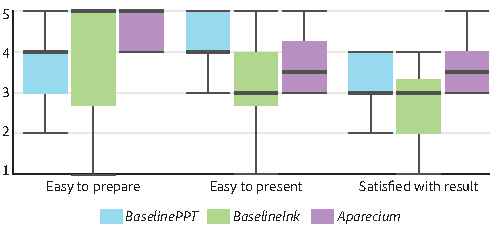
\includegraphics[width=0.8\textwidth]{figures/study1likert}
        \caption{Summary of Likert responses from Study 1 on a scale from 1 (strongly disagree) to 5 (strongly agree).}
\label{fig:likert}
\end{figure}
%
With Aparecium, most presenters did not do any extra work (revealing or writing beforehand) to set up the slides, but used them as-is. In the few cases, where they pre-revealed parts of the foreground, they expressed that the required effort was minimal.\\ 

In comparison, although our participants were familiar users of PowerPoint, they found the effort to set up animation effects tedious. To quote \textit{U6}, "\textit{It was cumbersome to add animations to each individual object and get the timing right... sometimes I decided I wanted to add an animation, but then had to figure out where to insert it in the existing animations sequence.}"\\

In terms of preparation effort, the BaselineInk condition was similar to our interface; most participants used the slide as-is, without writing additional content ahead of time. However, the reasons were different. In Aparecium, presenters had the ability to reveal the pre-authored foreground elements to the audience during the presentation. In the BaselineInk condition, presenters had to manually draw the foreground content, which they could either do ahead of time (thus losing the real-time effect) or during delivery. Either way, the effort was more \textit{"daunting"  (U12)} and  \textit{"time consuming" (U8)}, and the result was aesthetically less satisfactory (\textit{U1, U5, U8}).  
%%\val{Kruskall-Walis: chi-squared; 4.865, p = 0.0878}

\subsubsection{For presentation delivery, Aparecium involves comparable effort to BaselinePPT and less effort than BaselineInk.}
%{Kruskall-Walis chi squared: 4.044, p = 0.13}
%Presenters found it easiest to deliver the presentation using BaselinePPT, followed by our interface, and then BaselineInk.The difference between BaselinePPT and our interface (Mann-Whitney U test: Z = 1.18, p = .24) was less significant than between that of BaselinePPT and BaselineInk (Z = -1.88, p = .06). \\
%
Regarding the ease of delivering presentations, BaselinePPT received slightly higher ratings than our interface. BaselineInk was rated the lowest by a larger margin. 
%
It is not surprising that BaselinePPT required the least effort. The only interaction presenters used was to press a single button to advance the slide animations. That said, when the animation involved more than a few steps, it was common for presenters to make mistakes. 3 out of 12 participants forgot to advance the animation at the right time at least once, and only realized it at the next animation step. They had to either repeat the verbal explanation or quickly skip through the subsequent animations. In addition, two participants reported that they forgot to set up a desired animation step and only realized it during delivery. Several users suggested that having cues to help remember the animation would be beneficial $(U2, U7)$.\\

While presenters found inking in Aparecium straightforward, they noted that inking to reveal still required more effort than pushing a single button. Presenters seemed to prefer the path of minimum effort. For instance, with the exception of the math derivation content, they mostly used fast scribbling or strike-through gestures to reveal. As several presenters mentioned, this had the downside that the audience would initially see the scribbled ink strokes before the underlying pixels were revealed, which could potentially be distracting and aesthetically less pleasing. Some users suggested that they would prefer an even faster gesture such as clicking or circling to reveal large parts. On the other hand, they also expressed the idea that for the audience it could be better \textit{"to have the word appear after the inking instead of just after clicking like in powerpoint." (U1)} We discuss this tradeoff in more detail in the Limitations and Discussion section. In addition, users appreciated the automatic color selection for annotation and the modeless switching between revealing and inking. \\

As expected, BaselineInk required the most effort during delivery. Participants complained that drawing took away their attention from the content delivery. Since verbal explanations tend to be faster, there were periods of silence while the presenters were still drawing. In the Derivation presentation, three out of the four presenters who used BaselineInk ran out of space and had to use the margins or eraser. The one exception was a presenter who used the setup time to layout line numbers on the slide. In addition to these challenges, some users also complained about the specific difficulty of writing on a tablet. For example, the screen interface is not as smooth as paper \textit{(U1, U4, U6)} and operations such as switching to an eraser or a different color is tedious \textit{(U7, U9)}. 

\subsubsection{Presenters were most satisfied with the presentation quality of Aparecium.}
Presenters were most satisfied with the presentations produced using Aparecium. As shown in Figure~\ref{fig:likert}, the distribution of ratings for BaselinePPT was slightly lower, while BaselineInk was rated the lowest.
%
%The difference between our interface and BaselinePPT was less significant (Z = -0.95, p = .34) than that between ours and BaselineInk (Z = -1.88, p = 0.06). 
%
This trend held overall, as well as for each individual content type.\\

The feedback we gathered was consistent with our preliminary, formative interviews. Participants were accustomed to the BaselinePPT style, but in many cases they thought it could be improved with finer grained animation \textit{(U1, U3, U4, U8, U11)}. They liked the \textit{"handwritten in real time effect" (U4)}   in Aparecium, as it made the presentation \textit{"more interactive and seem to require engagement " (U9)}. The main complaints about BaselineInk presentations were that the drawings looked \textit{"messy" (U7)} and \textit{"not professional enough" (U6)}, and that the pace was too slow.\\

\subsubsection{Tool preference depends on presentation content.}
Figure~\ref{fig:votes} shows the preference data across content types from both studies. The tool preferences of both the presenters and audience depended on the content type.\\
%
\begin{figure}[h!]
    \centering
        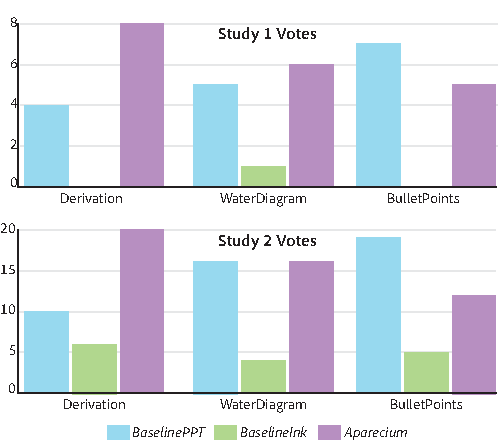
\includegraphics[width=0.8\textwidth]{figures/studyVotes}
        \caption{Preferred tool/presentation for each content type.}
\label{fig:votes}
\end{figure}
%

In Study 1, we asked presenters to choose which interface they would prefer to use for each content type.
For Derivation, presenters preferred  Aparecium (8/12) and then BaselineInk (4/12). For WaterDiagram, Aparecium (6/12) and BaselinePPT(5/12) were comparable choices. Similarly for BulletPoints, BaselinePPT (7/12) and Aparecium (5/12) were preferred.\\
%

In Study 2, we asked audiences which presentation was most engaging. For Derivation, the majority of audiences preferred Aparecium (20/36) followed by BaselinePPT (10/36) and then BaselineInk (6/36). For WaterDiagram, Aparecium (16/36) and BaselinePPT (16/36) were comparable. For BulletPoints audiences preferred BaselinePPT (19/36) and then Aparecium (12/36).\\

These findings confirm our intuition that fine-grained control of pace is most important for presenting sequential processes, especially for writing out text or equations (Derivation). In the case of the WaterDiagram, it was easy to achieve similar sized steps using BaselinePPT and Aparecium. The fact that the WaterDiagram slide consists mainly of images rather than text may have affected the users choice as well (see discussion about different ways to reveal). For simple lists and images (BulletPoint), BaselinePPT provided an appropriate pace and aesthetics.

%----------------------------------------------------------------------------------------

\section{Discussion}
Here, we consider some limitations of our design, and discuss several observations and lessons learned about designing future presentation interfaces.

\subsection{Limitations}
\subsubsection{Different Ways to Reveal.}  
Several presenters in the first user study wanted an even quicker way than scribbling to reveal content. Indeed, scribbling over large areas to reveal images or long lines of text can be tedious, especially if the presenter is not concerned about simulating the real-time hand-drawn effect. \\

In addition, some participants across both user studies complained that showing the scribbles before revealing the foreground elements is less aesthetically pleasing or even distracting. Conversely, other audience members commented that the scribbles served as helpful cues to draw attention to where information was about to appear.\\

In general, supporting different types of revealing mechanisms (e.g., clicking or lasso selection) and allowing instantaneous reveal of certain elements could improve the presentation experience. However, such a design should not increase the preparation effort or limit flexibility during presentation. For example, we considered allowing presenters to specify at setup time elements that can be revealed instantaneously upon clicking or tapping. However, this can make preparation tedious, akin to grouping elements and setting up animations in PowerPoint. Moreover, it does not allow presenters to change their mind during preparation about how to reveal elements. 

\subsubsection{Presenter Convenience vs. Presentation Quality.} 
The question of what revealing mechanisms to support points to a more fundamental tension with presenter interfaces. On the one hand, making the workflow more convenient for presenters is an important objective. However, it is at least as important to take into account the audience's point of view, since they are the intended consumers of the presentations themselves. For example, providing a larger set of revealing gestures may tempt presenters to always opt for the minimum-effort gesture at the cost of presentation quality. In fact, in an earlier prototype of our system, we allowed revealing either by lasso selection or slow tracing, and observed that presenters almost always opted for the lasso tool even for the \textit{Derivation} type of content, which compromised presentation quality for the audience. Instead, we opted for a design that \textit{forces} the presenter to go at a slower pace.\\

More broadly, designing presentation tools that achieve the right balance between the needs of presenters and audience members remains an interesting direction for future work. In this vein, previous research that systematically compares the effect of different presentation styles (e.g.,~\cite{seth2010powerpoint, cross2013typerighting}) may provide valuable guidance for new interfaces that assist and \emph{nudge} presenters towards the most effective communication techniques.

\subsubsection{Creating Flexible Interactivity.} 
Our work focuses on presenting slides with static visuals, and Aparecium supports limited interaction with the displayed content (i.e., shifting elements to create empty space). In our formative interviews, several participants expressed the desire to present interactive content that can be controlled on-the-fly, for instance, to explain the steps of a computer algorithm or a physics diagram. 
%
While there are many existing approaches to creating interactive diagrams, designing authoring and presentation tools that are both convenient and flexible is a challenging problem that bears further exploration.

\subsection{Conclusion}
This chapter introduced Aparecium, a novel presentation interface that combines inking interactions with pre-authored slides to help presenters deliver flexible and engaging presentations.\\

Our modeless inking interactions allow presenters to reveal, annotate and create extra space during a presentation. We evaluated our interface from the perspective of presenters and the audience by comparing it against two baseline interfaces, representing conventional slide and inking tools. Presenters found our interface easy to use both during preparation and delivery. In particular, for text-heavy, process-driven content, both presenters and audience preferred presentations delivered using Aparecium.\\ 

In light of these findings, we believe our inking interactions could be a valuable addition to existing slide-based presentation tools.


